% !TEX TS-program = xelatex
% !TEX encoding = UTF-8

% This is a simple template for a XeLaTeX document using the "article" class,
% with the fontspec package to easily select fonts.

\documentclass[11pt]{article} % use larger type; default would be 10pt

\usepackage{fontspec} % Font selection for XeLaTeX; see fontspec.pdf for documentation
\defaultfontfeatures{Mapping=tex-text} % to support TeX conventions like ``---''
\usepackage{xunicode} % Unicode support for LaTeX character names (accents, European chars, etc)
\usepackage{xltxtra} % Extra customizations for XeLaTeX
\usepackage{float}
%\setsansfont{Deja Vu Sans}
%\setmonofont{Deja Vu Mono}

% other LaTeX packages.....
\usepackage{geometry} % See geometry.pdf to learn the layout options. There are lots.
\geometry{a4paper} % or letterpaper (US) or a5paper or....
%\usepackage[parfill]{parskip} % Activate to begin paragraphs with an empty line rather than an indent

\usepackage{graphicx} % support the \includegraphics command and options

\title{Conclusion}
\author{Moncef BEN RAJEB}
%\date{} % Activate to display a given date or no date (if empty),
         % otherwise the current date is printed 

\begin{document}
\maketitle


 Suite à ce stage, j’arrive à la conclusion que travailler dans le domaine des réseaux sociaux est passionnant. C’est un domaine en évolution qui mènera toujours à de nouvelles problématiques très intéressantes.
Stample offre à ces futur utilisateurs un réseau social de qualité en ajoutant des fonctionnalités manquantes et améliorant l'ergonomie de l'apprentissage.
\paragraph{}
Ce stage m'a permis de consolider mes connaissances techniques et ma scalabilier.
Durant lequel, j'ai travaillé pour améliorer le système de login en ajoutant plus d'options le reset du mot de passe, la possibilité de crée un compte à partir d'une autres plateforme...
J'ai eu des sous tâches pour les notifications, les commentaires .J'ai pu résoudre les problèmes des membres développeur coté frontend.
 \paragraph{}
En dehors de Stampl,e j'ai enrichi mon Scala en suivant les cours sur Coursera et en faisant des exercices. Ces derniers sont disponibles \textit{sur mon compte GuitHub}\footnote{https://github.com/metanote}, pour deux raisons :
\begin{itemize}
\item La première d'apprendre les diffèrents outils du langage.
\item La deuxième pour améliorer mon Scala en s'adaptant à la programmation fonctionnelle.
\end{itemize}
Cela n'était pas évident pour moi, habitué à la pensée impérative, en outre je n'avais pas des bonnes connaissance en Lisp, Ruby, Clojure... Scala était le premier langage de son genre avec lequel j'ai débuté.
\paragraph{}
J'ai développé en plus ma première page web personnelle\footnote{http://ideas2d.com/moncef/home.php} en HTML5, ce projet à part entière est mis en ligne sur mon compte GuitHub, permettant ainsi à mes professeurs, mes collègues et mes amis de naviguer facilement pour découvrir un bon tutoriel Scala et de profiter de mes index disponibles en ligne. De plus, il est possible d’accéder aux sources, sur smon compte GuitHub\footnote{https://github.com/metanote/Summary-report}, pour me proposer des suggestions personnelles ou de m'envoyer des mails depuis cette page.
\paragraph{}
Pour la gestion du projet, j'ai découvert deux outils en ligne très efficaces :
-Flowdock qui ne permet pas seulement d'avoir un système de "chat" en ligne avec les membres de l'équipe mais aussi de voir l'avancement du projet git instantanément et qui s'intègre aussi trello.
-Ce dernier c'est un outil permettant d'attribuer des tâches aux différents membres de l'équipe, de suivre l'historique, l'avancement d'un projet en ajoutant des cartes aux développeurs Frontend ou Backend comme (doing, done and later) et d'assigner chacun à ces cartes.
Personnellement, je trouve cet outil plus efficace qu'un gestionnaire de tâches classiques comme Gant \footnote{http://www.ganttproject.biz/}…
\paragraph{}
Cette expérience s’est avérée très intéressante, dans le sens où j’ai pu participer à des réunions, qui m’ont fait connaitre les contraintes et les avantages du travail en groupe.
En dehors de ces bénéfices plus ou moins attendus, j'ai appris un vocabulaire de Startup : Lever de fonds, Investisseurs … et par conséquence j'ai eu l'envie de lancer ma propre Startup plus tard.
\section{Critiques}

Ce Stage était un premier pas relativement dure dans la vie professionnelle pour des multiples raisons :
\begin{itemize}
\item Apprendre Scala et avancer dans le sujet simultanément.

\item Ecrire du code dans un Backend existant.

\item Connaitre les plugins du Backend comme Salat…

\item Utiliser une base de donnée NoSQL.

\item Je n'ai pas pu écrie aucune ligne de code dans le Linked Data Platform banana-rdf\footnote{https://github.com/stample/banana-rdf}.

\item J'ai seulement tester le Read Write Web play rww-paly\footnote{https://github.com/stample/rww-play}.



\end{itemize}

Ces deux derniers points peuvent être des nouveaux objectifs au cours de mon deuxième année master vu que les deux bibliothèques open source sont disponible sur GuitHub.  

\newpage
\section{Annexe}

\textbf{https://stample.co/login} my Stample Profile.
\begin{figure}[H]
        \centering
                \centering
                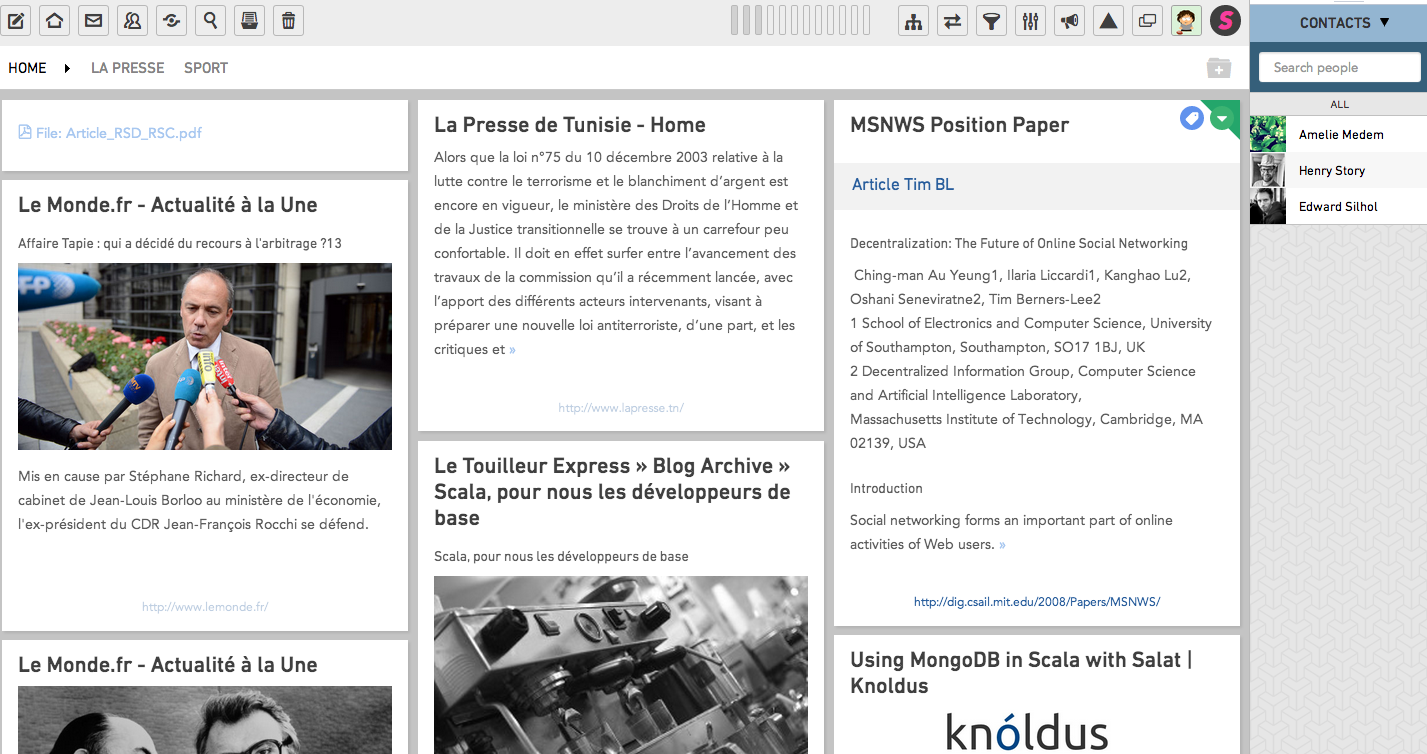
\includegraphics[width=\textwidth]{Stample.png}
		\caption{}

               
\end{figure}

\textbf{https://www.flowdock.com/} my Flowdock workspace Profile.
\begin{figure}[H]
        \centering
                \centering
                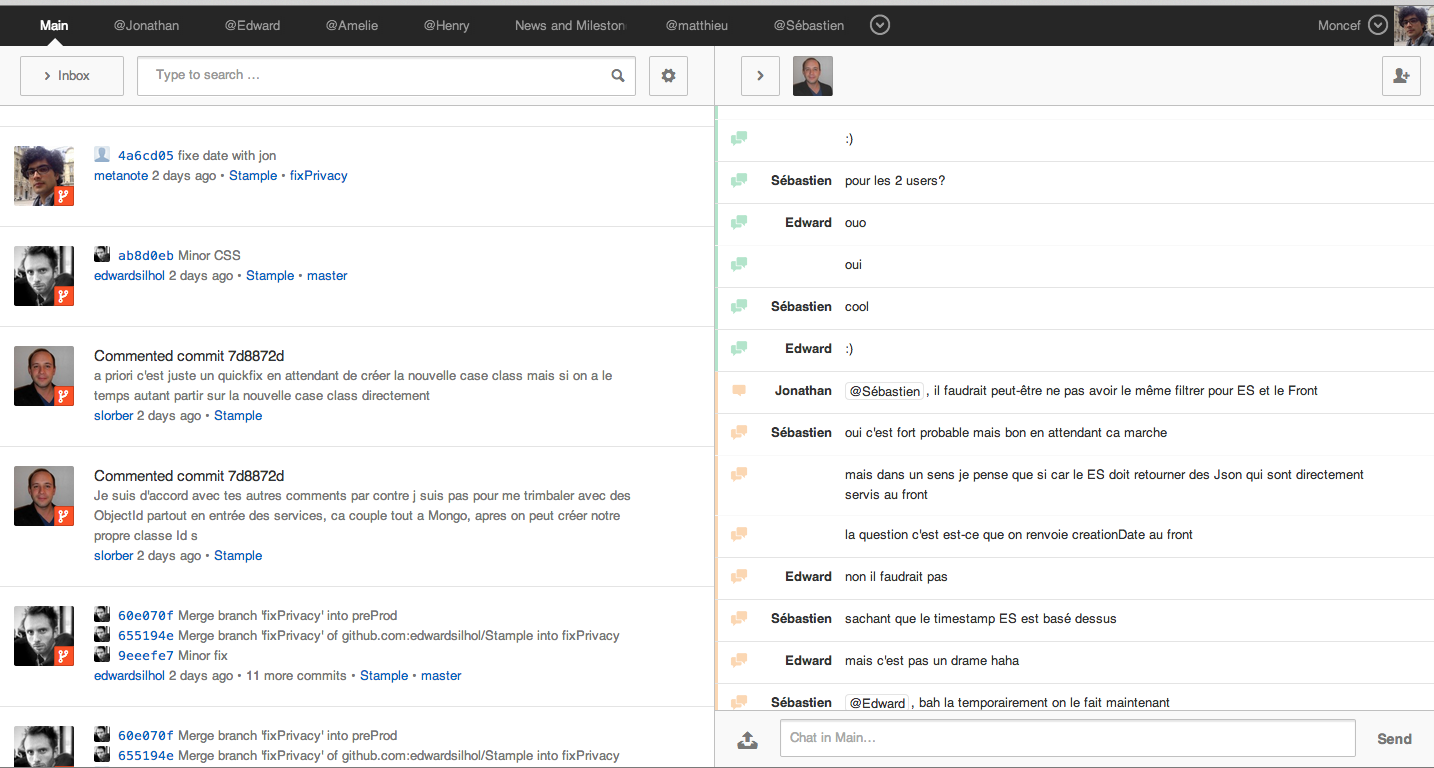
\includegraphics[width=\textwidth]{Flowdock.png}
               
\end{figure}
\newpage
\textbf{https://stample.co/login} my Trello workspace Profile.
\begin{figure}[H]
        \centering
                \centering
                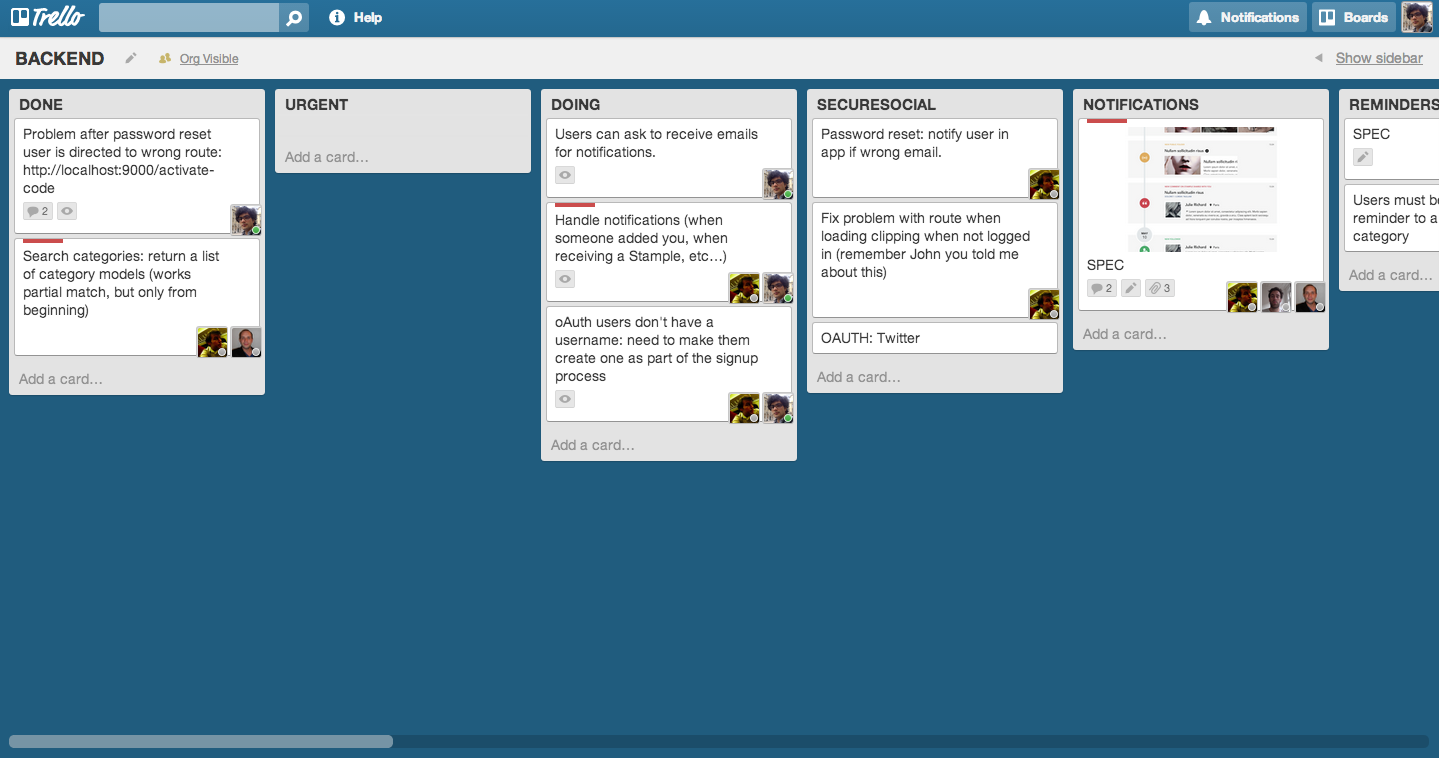
\includegraphics[width=\textwidth]{trello.png}
               
\end{figure}

\end{document}
